\chapter{Modello del sistema}

\thispagestyle{empty}

\begin{figure}[ht]
    \centering
    \begin{tikzpicture}[scale=0.65,>=latex]
    \tikzstyle{every node}=[font=\fontsize{9}{9}\sffamily]

    \draw[->] (0,0) -- (20,0) node[right]{$f$};

    \filldraw[
        fill=nord10!75!nord4,
        draw=nord10!50!nord0
    ] (1,0) rectangle (8,4)
    node[nord6,midway]{\bfseries Uplink};
    \filldraw[
        fill=gray,
        draw=darkgray
    ] (2,0) rectangle (3.2,2.5);
    \draw[->] (1.5,1) -- (2,1);
    \draw[<-] (3.2,1) -- (3.7,1) node[right,align=left]{
        \scriptsize Larghezza di banda \\ \scriptsize del sistema
    };
    \draw[Red,semithick] (2.6,0) -- (2.6,5) node[Black,above]{
        \(f_\mathrm{UL}\)
    };

    \draw[<->] (1,-0.4) -- (8,-0.4)
    node[below,midway]{Larghezza di banda alloccata};

    \filldraw[
        fill=nord14!90!nord3,
        draw=nord14!50!nord0
    ] (12,0) rectangle (19,4)
    node[nord6,midway]{\bfseries Downlink};
    \filldraw[
        fill=gray,
        draw=darkgray
    ] (13,0) rectangle (14.2,2.5);
    \draw[Red,semithick] (13.6,0) -- (13.6,5) node[Black,above]{
        \(f_\mathrm{DL}\)
    };

    \draw[<->] (8,2) -- (12,2) node[below,midway]{Banda proibita};

    \draw[<->] (2.6,5) -- (13.6,5) node[above,midway]{Spaziatura duplex};
\end{tikzpicture}

    \caption{Struttura tipica dei moderni sistemi cellulare FDD.}
    \label{fig:fdd-system}
\end{figure}

Consideriamo il sistema cellulare in modalità FDD illustrato in
Figura~\ref{fig:fdd-system}, dove \(f_\mathrm{UL}\) e \(f_\mathrm{DL}\)
denotano le frequenze della portante centrale di UL e DL, rispettivamente.
Assumiamo che la BS comunichi con diversi UTs e che tutti i dispositivi siano
dotati di una singola antenna.

In questa trattazione ci concentriamo su una trasmissione multiportante a
singola antenna, implementata, ad esempio, con \textit{orthogonal
frequency-division multiplexing} (\textit{OFDM}, multiplex a divisione di
frequenze ortogonali) e \textit{single-carrier frequency-division multiple
access} (\textit{SC-FDMA}, accesso multiplo a divisione di frequenza a singola
portante) per le trasmissioni in DL e UL, rispettivamente, così come nello
standard \textit{Long-Term Evolution} (\textit{LTE}). Si noti che le
derivazioni riportate e le tecniche proposte si applicano anche ad altri
contesti, come ad esempio scenari \textit{multiple-input multiple-output}
(\textit{MIMO}) a banda stretta dove i canali sono descritti da matrici che
delineano i collegamenti tra coppie di antenne. Nella nostra situazione, i
canali di UL e DL sono entrambi descritti da \(N/2\) numeri complessi (con
\(N\) pari), ognuno denotante il coefficiente di una sottoportante
OFDM.\footnotemark

\footnotetext{Si noti che in un contesto MIMO la dimensione dei due vettori
potrebbe essere differente. È il caso ad esempio di uno scenario
\textit{multi-user MIMO} (\textit{MU-MIMO}), nel quale una BS con \(M\) antenne
serve \(K\) UTs a singola antenna, e tipicamente si ha \(M \gg K\) di modo da
poter servire più utenti o operare meglio alle frequenze delle onde
millimetriche. Ad ogni modo, le derivazioni riportate non dipendono dalla
dimensione dei due vettori e possono essere facilmente generalizzate.}

Il canale aggregato UL-DL è descritto da un vettore di \(N\) numeri complessi.
Ci concentriamo sul problema dell'acquisizione del canale di DL alla BS, e
assumiamo che questa acquisizione avvenga in momenti diversi per ognuno degli
UT. Restringiamo il nostro studio al caso in cui un solo UT è presente nel
sistema. Denotiamo i vettori dei canali di UL e DL come
\begin{equation}
    \begin{aligned}
        \bm{h}^\mathrm{(U)} &= \mleft[
            h_0^\mathrm{(U)}, \dots, h_{N/2-1}^\mathrm{(U)}
            \mright] \in \C^{1 \times N/2},\\
        \bm{h}^\mathrm{(D)} &= \mleft[
            h_{N/2}^\mathrm{(D)}, \dots, h_{N-1}^\mathrm{(D)}
            \mright] \in \C^{1 \times N/2},
    \end{aligned}
\end{equation}
e il vettore del canale globale come
\begin{equation}
    \bm{h} = \mleft[
        \bm{h}^\mathrm{(U)}, \bm{h}^\mathrm{(D)}
        \mright] \in \C^{1 \times N}.
\end{equation}
In generale, i canali di UL e DL sono in relazione tra loro, dal momento che
hanno origine dallo stesso canale fisico. Infatti, i fenomeni fisici (quali, ad
esempio, la riflessione, la dispersione e l'assorbimento) che determinano il
canale a una data frequenza hanno un comportamento simile a frequenze vicine.
Questo risulta particolarmente vero per un canale con solo pochi dispersori,
come ad esempio un canale a onde millimetriche. In generale, poiché il segnale
ricevuto alla BS e allo UT viene in entrambi i casi normalizzato a una data
potenza adeguata per eseguire la quantizzazione, assumiamo che sia
\(\bm{h}^\mathrm{(U)}\) che \(\bm{h}^\mathrm{(D)}\) abbiano norma unitaria,
ovvero,
\begin{equation}
    \lnorm \bm{h}^\mathrm{(U)} \rnorm^2 = 1, \quad
    \lnorm \bm{h}^\mathrm{(D)} \rnorm^2 = 1.
\end{equation}

In alcuni casi, come ad esempio nello standard LTE, il feedback del
coefficiente di normalizzazione viene effettuato del segnale di
\textit{channel-quality information} (\textit{CQI}, informazione sulla qualità
del canale); per cui, possiamo considerare il problema del feedback della norma
come a sé stante.\footnotemark

\footnotetext{Si noti che in un contesto MIMO massivo, l'effetto di indurimento
del canale può anch'esso essere sfruttato per recuperare l'informazione
riguardo la norma del canale.}

Assumiamo inoltre che, all'inizio della trasmissione, la BS trasmetta un numero
sufficiente di simboli pilota affinché lo UT possa ottenere una stima perfetta
del canale di DL e, allo stesso modo, lo UT trasmetta sufficienti simboli
pilota di modo che la BS ottenga una perfetta stima del canale di UL.

Il problema affrontato è come ottenere una stima del canale di DL alla BS,
tramite uno scambio di comunicazioni con lo UT. Alla BS, questa conoscenza
viene poi utilizzata per il bit- e power-loading delle sottoportanti e/o per il
beamforming quando più antenne vengono utilizzate. Quindi, la nostra attenzione
è sia sulle strategie di segnalazione che sulla quantizzazione vettoriale di
\(\bm{h}^\mathrm{(U)}\) e \(\bm{h}^\mathrm{(D)}\), denotate rispettivamente
come
\begin{equation}
    q(\bm{h}^\mathrm{(U)}), \quad q(\bm{h}^\mathrm{(D)}),
\end{equation}
utilizzando il minor numero di bit possibile nello scambio di informazioni tra
BS e UT. L'approccio considerato in questa trattazione utilizza il feedback del
CSI a tasso variabile. In questo caso, la BS non effettua una segnalazione in
feedforward, mentre il segnale di feedback che viene trasmesso dallo UT
utilizza un numero variabile di bit ed è ottenuto tramite uno schema di
codifica entropica Slepian-Wolf basato sul lavoro di Al Jabri e
Al-Issa.\cite{10.1007/BFb0024445}

Come misura di distorsione, utilizziamo l'\textit{errore quadratico medio
normalizzato} (\textit{NMSE}, dall'inglese ``normalized mean squared error'')
dell'errore di quantizzazione, ovvero,
\begin{equation} \label{eq:nmse}
    \mathrm{NMSE} = \expect{
        \lnorm \bm{h}^\mathrm{(D)} - q(\bm{h}^\mathrm{(D)}) \rnorm^2
    },
\end{equation}
dove la normalizzazione fa riferimento al fatto che \(\bm{h}^\mathrm{(D)}\) è
stato normalizzato a norma unitaria. Per cui, la \eqref{eq:nmse} può anche
essere interpretata come \textit{errore quadratico medio} (\textit{MSE}) per
componente vettoriale. Si noti che questa definizione differisce da altre
comunemente definite come MSE normalizzato.

\begin{figure}[ht]
    \centering
    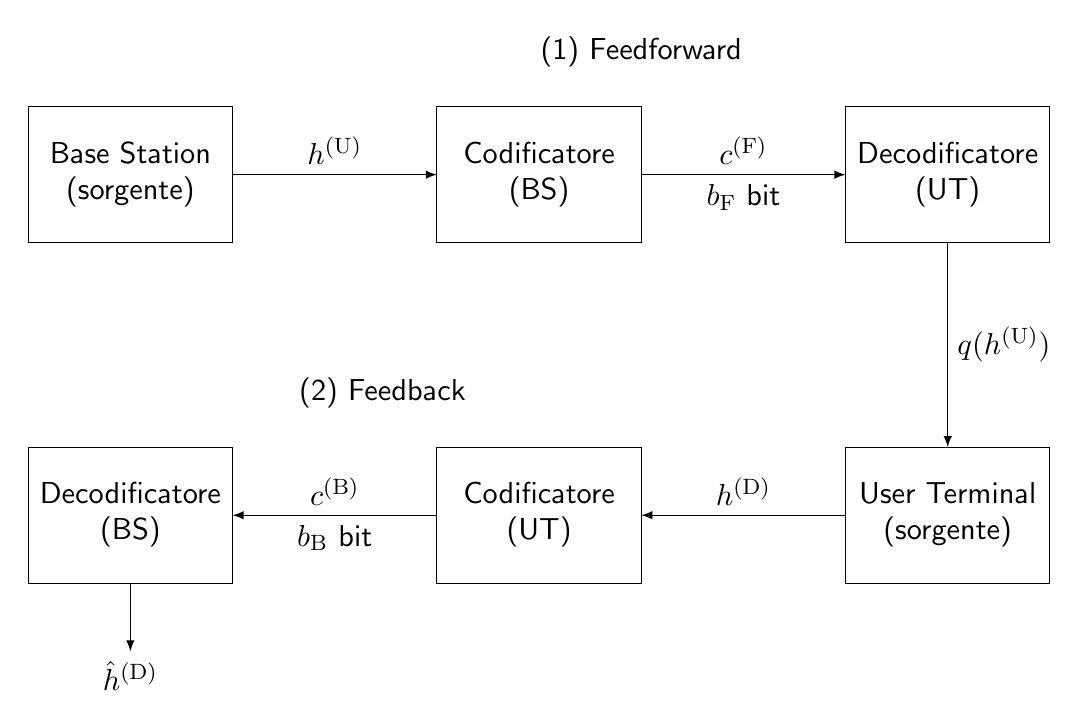
\begin{tikzpicture}[scale=0.865,>=latex]
    \tikzstyle{every node}=[font=\fontsize{11}{13}\sffamily]

    % Bottom Half

    \node at (5.2,2.8) {(2) Feedback};

    \draw[->] (1.5,0) -- (1.5,-1)
    node[below]{\(\hat{\bm{h}}^\mathrm{(D)}\)};

    \draw (0,0) rectangle (3,2)
    node[midway,align=center]{Decodificatore \\ (BS)};

    \draw[->] (6,1) -- (3,1)
    node[above,midway]{\(c^\mathrm{(B)}\)}
    node[below,midway]{\(b_\mathrm{B}\) bit};

    \draw (6,0) rectangle (9,2)
    node[midway,align=center]{Codificatore \\ (UT)};

    \draw[->] (12,1) -- (9,1)
    node[above,midway]{\(\bm{h}^\mathrm{(D)}\)};

    \draw (12,0) rectangle (15,2)
    node[midway,align=center]{User Terminal \\ (sorgente)};

    % Top Half

    \node at (9,7.8) {(1) Feedforward};

    \draw[->] (13.5,5) -- (13.5,2)
    node[right,midway]{\(q(\bm{h}^\mathrm{(U)})\)};

    \draw (12,5) rectangle (15,7)
    node[midway,align=center]{Decodificatore \\ (UT)};

    \draw[->] (9,6) -- (12,6)
    node[above,midway]{\(c^\mathrm{(F)}\)}
    node[below,midway]{\(b_\mathrm{F}\) bit};

    \draw (6,5) rectangle (9,7)
    node[midway,align=center]{Codificatore \\ (BS)};

    \draw[->] (3,6) -- (6,6)
    node[above,midway]{\(\bm{h}^\mathrm{(U)}\)};

    \draw (0,5) rectangle (3,7)
    node[midway,align=center]{Base Station \\ (sorgente)};
\end{tikzpicture}

    \caption{
        Schema del sistema Base Station-User Terminal con fasi di
        codifica/decodifica dei canali di Uplink e Downlink. Per la descrizione
        delle variabili di feedforward \(c^\mathrm{(F)}\) e feedback
        \(c^\mathrm{(B)}\) si veda l'Appendice~\ref{app:codebook-design}.
    }
    \label{fig:complete-schema}
\end{figure}
